\documentclass[a4paper, 12pt]{article}
\usepackage[utf8]{inputenc}
\usepackage[left=2cm,right=2cm,top=2cm,bottom=2cm]{geometry}
\usepackage[pdftex]{graphicx}
\usepackage[final]{pdfpages}
\usepackage{color}

\begin{document}
\begin{titlepage}
\begin{center}

\includegraphics[scale=1.50]{UMONS.jpg}\\[0.4cm]

\includegraphics[scale=0.30]{FS_Logo.jpg}\\[3cm]
{\huge Réseayx II - TP3}\\
\vspace{0.9mm}
\rule{9.5cm}{0.5mm}\\[0.5cm]
{\huge \bfseries Tiny Internet Project}\\[0.2cm]
\rule{9.5cm}{0.5mm}\\[7cm]
      \begin{flushleft} \large
        Jason \textsc{Bury} 130538\\
        Alicia \textsc{Galina} 130852\\
        Master 1 en Sciences informatiques\\
      \end{flushleft}
   \vfill
  {\large 11/11/2016}
\end{center}
\end{titlepage}

\section{Introduction}
Le but du projet est de simuler la topologie de la figure \ref{topo} avec l'outil cbgp et ensuite de configurer chaque routeur comme étant un routeur BGP et de créer des filtres pour chaque routeur.
Pour chaque filtre, on réfléchit pour servir uniquement les intérêts de l'AS en question.
\\

Pour inclure tous les fichiers via l'invite de commande cbgp, il suffit d'inclure le fichier tinyWeb.cli.
Ensuite, il faut taper \texttt{sim run} pour que les routes se transmettent.

\begin{figure}
 \fbox{
 \begin{minipage}[c]{.25\linewidth}
  \begin{center}
   \textbf{Légende}
  \end{center}
  \begin{itemize}
   \item {\color{red} Rouge}:\\Relation\\commerciale\\(profit).
   \item {\color{green} Vert}:\\Relation\\gouvernementale\\(sans profit).
  \end{itemize}
 \end{minipage}
 }
 \begin{minipage}[c]{.75\linewidth}
  \centering
  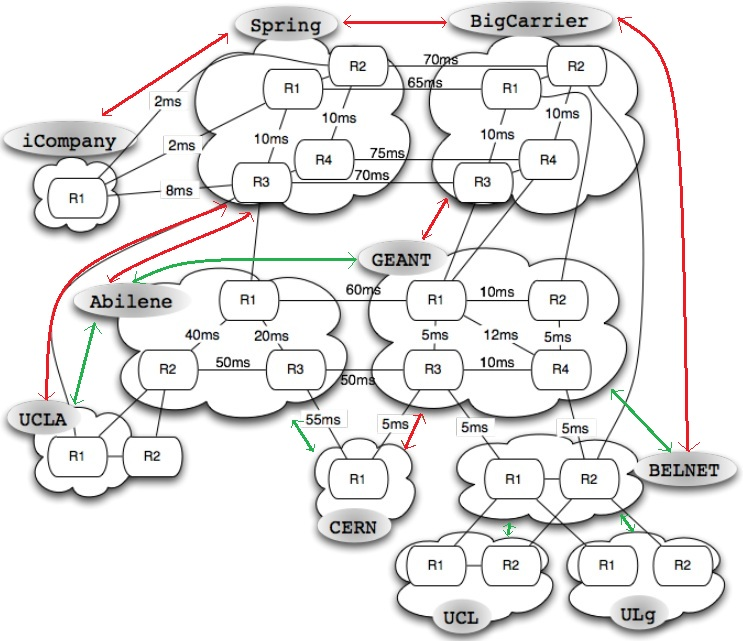
\includegraphics[scale=0.65]{businesstiny.jpg}
 \end{minipage}
 \label{topo}
 \caption{Topologie et relations business}
\end{figure}

\section{Filtres}
Un client paie à son fournisseur la bande passante utilisée sur le(s) lien(s) qui les connecte(nt), peu importe le sens du trafic.
De plus, certaines routes sont à préférer à d'autres pour des questions de latences (affiché en ms sur chaque lien dans la figure \ref{topo}).
\subsection{Règles générales}
Voici quelques raisonnements utilisés pour plusieurs AS:
\begin{enumerate}
 \item Si on a plusieurs fournisseurs, on fait en sorte que les routes annoncées par un fournisseur ne soient pas annoncées à un autre.
 Sinon, le fournisseur qui reçoit la route pourra faire passer du trafic par chez nous pour atteindre l'autre fournisseur.
 \item Si on a un lien peer avec un autre AS, ne pas annoncer les routes venant de cet AS aux fournisseurs.
 \item Soit B client de A, C client de B et C client de A, A voudrait que le trafic à fournir à C évite de passer par B. %%c'est pas la meme chose pour lui? il s'en fout non? fin du moment que le client paie, il preferera celui qui paie le plus cher non? (et sinon avec l'as-path ca mettra le plus court direct) 
 \item Pour les réseaux gouvernementaux, ne pas annoncer les routes vers les fournisseurs payant aux clients et inversément.
\end{enumerate}

\subsection{UCLA}
J'applique la règle 1.
En effet, nous ne voulons pas que Spring transmettent des paquets à Abilene en utilisant UCLA comme intermédiaire (et inversement).
Pour ce faire, pour chaque routeur j'indique qu'aucune route ne doit être annoncée aux fournisseurs sauf celles dont le préfixe correspond au réseau UCLA.

\subsection{CERN}
Règle 1 appliquée. De plus,
imaginons qu'un AS doit nous transmettre des paquets et qu'il a plusieurs choix de route : une passant par GEANT et l'autre par Abilene.
Alors, on voudra faire en sorte que cet AS préfère la route passant par Abilene puisque GEANT fourni un transit commercial et pas Abilene.
On aura alors moins de bande passante à payer à GEANT.
\\

On va donc ajouter le numéro d'AS de CERN beaucoup de fois dans l'AS-PATH passant par GEANT pour que ces routes soient très défavorisées.
En effet, habituellement, un routeur BGP préviligiera les routes dont l'AS-PATH est le plus court. 
\\

On va aussi également configurer une préférence plus élevée pour les routes communiquée par Abilene.
Cette fois-ci ce sera la commande \texttt{local-pref} qui sera utilisée.

\subsection{BELNET}
Règle 1 appliquée.

\subsection{UCL}
UCL n'a qu'un seul fournisseur. Donc il n'y a pas de danger si on annonce n'importe quelle route au fournisseur.
Si UCL annonce une route venant de BELNET à BELNET, il ne devra normalement pas faire passer de paquet par UCL pour, par exemple, transfèrer un paquet de R1 de BELNET à R2 de BELNET.
En effet, les implémentations habituelles de routeur BGP lisent l'AS-PATH pour tester si son propre numéro d'AS ne s'y trouve pas.
Et si il s'y trouve, la route n'est pas communiquée sinon cela créerait une boucle.
Néanmoins, par prudence, nous allons quand-même configurer les filtres comme chez UCLA.

\subsection{ULg}
Le raisonnement à avoir est exactement le même que pour UCL.

\subsection{Abilene}
Règle 2 et 4 appliquées. Toutes les routes venant de GEANT ne doivent pas être transmises à Spring.
Toutes les routes venant de Spring ne doivent pas être transmises à UCLA et CERN.
Et inversément, les routes venant de UCLA et CERN ne doivent pas être annoncées à Spring.

\subsection{GEANT}
Règle 2 et 4 appliquées. Toutes les routes venant de Abilene ne doivent pas être transmises à BigCarrier.
Toutes les routes venant de BigCarrier ne doivent pas être transmises à Belnet et toutes les routes venant de BELNET ne doivent pas être annoncées à BigCarrier.
Mais on annonce néanmoins ces routes à CERN, vu l'exception.

Et de plus, on sait que CERN a Abilene comme fournisseur sans but lucratif. %% est ce qu'il en est reellement concient? (nous oui vu qu'on voit le dessin mais pour Geant est-ce qu'il n'a pas connaissance que de ses propres liens?
On suppose donc que CERN va essayer de favoriser les routes passant par Abilene.
On va donc éviter cela en annonçant pas à BELNET les routes passant par CERN et Abilene.
Cela est possible grâce à la commande \texttt{path RE} de CBGP.

\subsection{Spring} %besoin de filtre?
Spring n'a pas de fournisseur et donc il n'est pas nécessaire d'appliquer la règle 2.
\\

En revanche, la règle 3 est applicable.
Mais elle sera d'office respéctée puisque les routes passant par UCLA et Abilene auront un AS-PATH plus grand que les routes à même destinations passant par UCLA mais pas Abilene.
Et que donc le routeur privilégiera la route ne passant pas par Abilene.
\\

Les algorithmes de plus court chemin appliqués sur chaque routeur ne prennent pas en compte les nœuds internes aux AS étrangers.
C'est pour cela que si iCompany doit transmettre un paquet passant par Abilene, il ne l'envoie pas à R3 de Spring via le lien de latence 8ms.
(Avec la commande traceroute, on observe que le lien utilisé est un lien à 2ms vers R1 de Spring)
On va donc privilegier ce lien à 8ms en ajoutant le numéro d'AS de Spring 2 fois dans l'AS-PATH au lien de 1 fois pour les routes transmisent par R1 et R2 de Spring.

\subsection{BigCarrier}%besoin de filtre?
Il n'est pas nécessaire d'appliquer la règle 2 puisque BigCarrier n'a pas de fournisseur.
La règle 3 est applicable et appliquée d'office, normalement.

\end{document}
